\documentclass{article}
\usepackage{graphicx} % Required for inserting images
\usepackage[spanish]{babel}
\usepackage{float}
\usepackage{minted}
\usepackage{listings}
\usepackage{xcolor}
\usepackage{hyperref}

\lstset{
    language=bash,
    basicstyle=\ttfamily\small,  % Tipo de letra monoespaciada
    keywordstyle=\color{blue},   % Color de palabras clave
    stringstyle=\color{red},     % Color de strings
    commentstyle=\color{gray},   % Color de comentarios
    showstringspaces=false       % No mostrar espacios en strings
}

\lstdefinelanguage{SQL}{
    keywords={SELECT, FROM, WHERE, INSERT, INTO, VALUES, UPDATE, SET, DELETE, CREATE, TABLE, ALTER, DROP, INDEX},
    keywordstyle=\color{blue}\bfseries,
    morekeywords={PRIMARY, KEY, FOREIGN, NOT, NULL, AUTO_INCREMENT, DEFAULT, CONSTRAINT},
    sensitive=false,
    morestring=[b]',
    morecomment=[l]--,
    morecomment=[s]{/*}{*/},
    commentstyle=\color{gray}\ttfamily,
    stringstyle=\color{red}\ttfamily,
}

\begin{document}

% Portada
\begin{titlepage}
    \centering
    
\includegraphics[width=0.4\textwidth]{logo.png} % Ajusta el nombre de la imagen según corresponda
    \\[2cm]
    {\Huge \textbf{Práctica 1: Grafana}}\\[1.5cm]
    {\Large \textit{Evaluación de Sistemas Informáticos}}\\[1cm]
    {\large 3º Grado en Informática. Mención de TI}\\[1cm]
    {\large Grupo 6}\\[1.5cm]
    \textbf{Autores:}\\[0.7cm]
    Víctor Fernández Sánchez\\
    Gonzalo Sánchez Maroto\\
    Diego Sanz Santos\\
    Rubén Verduras Cavada\\[2cm]
    \vfill
    \today
\end{titlepage}

\tableofcontents % Componer y mostar el índice
\listoffigures % Componer y mostrar el índice de tablas
\listoftables % Componer y mostrar el índice de figuras
\newpage

\section{¿Qué es Grafana?}

Grafana es un software de código abierto que permite consultar, visualizar, alertar y comprender datos en tiempo real sin importar dónde estén almacenados mostrados a través de paneles elegantes y flexibles.

Las principales características de Grafana son:

\begin{itemize}
    \item Permite crear dashboards altamente interactivos con gráficos y tablas que se pueden personalizar y explirar en tiempo real.
    \item Admite una amplia variedad de fuentes de datos como bases de datos SQL y NoSQL, sistemas de monitoreo como Prometheus y Graphite y sistemas en la nube como AWS CloudWatch y Google Stackdriver.
    \item Ofrece una amplia gama de opciones de visualización como gráficos de líneas, barras, dispersión, termómetros y más.
    \item Aporta la posibilidad de crear alertas basadas en umbrales y condiciones definidas por los usuario capaces de notificar a través de correo electrónico u otros canales de comunicación.
    \item Facilita la exploración y análisis de datos mediante funciones de búsqueda, filtrado y agregación, que permite a los usuarios investigar tendencias y patrones en los datos.
    \item Altamente seguro con sistemas basados en autenticación de usuarios y controles de acceso a datos basados en roles.
\end{itemize}

Según estas características algunos casos de uso son los siguientes:

\begin{enumerate}
    \item Monitoreo de infraestructura: supervisar el rendimiento de servidores, redes y bases de datos, identificando problemas y optimizando recursos.
    \item Visualización de métricas de aplicaciones: rastrea el rendimiento, identifica cuellos de botella y mejora la experiencia del usuario.
    \item Análisis de registros: correlacionar datos de registros con métricas para investigar problemas y tendencias en sistemas distribuidos.
    \item Observabilidad de microservicios: monitorizar la salud y rendimiento de estos para identificar problemas de comunicación entre servicios.
    \item Seguridad informática: visualizar datos de seguridad, como registros de acceso, eventos de autenticación y actividad sospechosa, para detectar y responder a las amenazas de manera más eficiente.
\end{enumerate}

\section{Instalación Grafana}

Para realizar la instalación de Grafana en su versión Standalone Linux Binaries, se ejecutaron los siguientes comandos, que descargarán y descomprimirán el archivo respectivamente:

\begin{minted}{bash}
- wget https://dl.grafana.com/enterprise/release/grafana-
enterprise-11.5.2.linux-amd64.tar.gz
- tar -zxvf grafana-enterprise-11.5.2.linux-amd64.tar.gz
\end{minted}

Una vez descomprimido todo se debe de iniciar el servidor con el comando \lstinline[language=bash]|stemctl start grafana-server.service| 
y podemos confirmar que se ha iniciado si ejecutamos \lstinline[language=bash]|systemctl status grafana-server.service|.\\

Con el servidor de Grafana en funcionamiento, se puede acceder a este mediante la URL  ''http://virtual.lab.inf.uva.es:31222'' (en nuestro caso).

\section{Base de datos}

Grafana necesita estar conectada a una base de datos para poder crear sus tablas y esquemas para mostrar los valores que se almacenan en ellas. Utilizaremos MySQL, en donde Grafana puede utilizarlo de dos maneras distintas:

\begin{itemize}
    \item Como base de datos interna de Grafana, para usuarios y permisos, dashboards y paneles o ajustes o auditorías.
    \item Como fuente de datos externa, en donde Grafana realizará consultas SQL a los datos y creará gráficos para mostrarlos, construyendo así dashboards dinámicos.
\end{itemize}

En nuestra práctica hemos conectado una base de datos MySQL llamada ''grafana'' con URL host ''localhost:3306'' debido a que 3306 es el puerto predeterminado de MySQL.

\newpage
\subsection{Esquema entidad relación}
Aquí podríamos explicar el esquema E/R y la estructura de la bbdd cuando esté completa.
\newpage

\subsection{Conexión a la base de datos}\label{subsec:conexión-db}
Este código define una conexión con la base de datos \textbf{MySQL} en Ubuntu. El script está desarrollado en Python y maneja tanto la conexión con la base de datos como su cierre.

\begin{minted}{python}
def get_connection():

    try:
        host = "localhost"
        port = 3306
        database = "grafana"
        user = "grafanareader"
        password = "Grupo6esi"
        
        connection = pymysql.connect(
            host=host,
            port=port,
            database=database,
            user=user,
            password=password,
            charset='utf8mb4',  # Evita problemas de encoding
            cursorclass=pymysql.cursors.DictCursor
        )
        return connection
    except pymysql.MySQLError as e:
        print("Error al conectarse a la base de datos:", e)
        return None

def close_connection(connection):

    if connection:
        connection.close()
\end{minted}

Explicación:

\begin{itemize}
    \item \textbf{get\_connection()}: Establece una conexión con la base de datos MySQL. Para ello, se deben especificar el \textit{host, puerto, nombre de la base de datos, usuario y contraseña}. Retorna un objeto de conexión \textbf{pymysql.connections.Connection} si la conexión es exitosa; en caso contrario, retorna \textbf{None}.
    \item \textbf{close\_connection()}: Cierra una conexión existente con la base de datos. Requiere como parámetro un objeto de conexión \textbf{pymysql.connections.Connection} que será cerrado.
\end{itemize}

\subsection{Iniciar la base de datos en el servidor}

Para iniciar la base de datos en el servidor es necesario acceder como root con el comando \lstinline{sudo -i}. A continuación ejecutamos los siguientes comandos:

\begin{itemize}
    \item \lstinline{mysql} $ \rightarrow $ abre el cliente de línea de comandos de MySQL, permitiendo interactuar con la base de datos.
    \item \lstinline{use grafana} $ \rightarrow $ selecciona la base de datos llamada 'grafana' para que todas las operaciones posteriores se ejecuten sobre ella.
    \item \lstinline{source /home/usuario/esi/db/tablasGrafana.sql;} $ \rightarrow $ ejecuta el archivo SQL que contiene las instrucciones para crear las tablas y almacenar datos en la base de datos 'grafana'.
\end{itemize}

\section{Servicio de Ubuntu}\label{sec:servicio-ubuntu}
Este código define un servicio de \textbf{systemd} de Ubuntu, que ejecuta un script desarrollado en python3 dedicado a la recolección de datos del servidor y enviarlos a Grafana. El servicio depende de MySQL y se reinicia automáticamente si falla.
Este código se encuentra dentro de \textbf{/etc/systemd/system/} con el nombre de \textbf{programa-grupo6.service}.

\begin{minted}{bash}
[Unit]
Description=Daemon programa esi
After=network.target
After=mysql.service
Requires=mysql.service

[Service]
ExecStart=/usr/bin/python3 /home/usuario/esi/script/script_grafana.py
WorkingDirectory=/home/usuario/esi
Restart=always
User=usuario
Group=usuario

[Install]
WantedBy=multi-user.target 
\end{minted}

Explicación:

\begin{itemize}
    \item \textbf{[Unit]} $ \rightarrow $ define la descripción y dependencias del servicio. Indica que se ejecuta después de que la red y MySQL estén activos.
    \item \textbf{[Service]} $ \rightarrow $ especifica el comando para iniciar el script, su directorio de trabajo y que se reiniciará en caso de fallo. Además, se ejecutará con el usuario \textit{usuario}.
    \item \textbf{[Install]} $ \rightarrow $ indica que el servicio debe ejecutarse en el nivel \textit{multi-user.target}.
\end{itemize}

\section{Explicación del código}
\subsection{Bucle while del servicio}\label{subsec:bucle-while}

\begin{minted}{python}
conn = None

try:
    
    conn = get_connection()

    if conn:
        print("Conexión a la base de datos establecida correctamente")

        """Ejecuta la recolección de datos e inserción en la BD en intervalos regulares"""
        while True:
            data = collect_data()
            if data:
                insert_data(data, conn)

            time.sleep(5)  # Espera 10 segundos antes de la siguiente medición
except Error as e:
    print(f"Error al conectar bas de datos: {e}")
finally:
    if conn:  # Si la conexión fue establecida, cierra la conexión
        close_connection(conn)  # Cerrar la conexión al finalizar el programa
\end{minted}

Explicación:

\begin{itemize}
    \item \textbf{Establecimiento de conexión}: Se establece la conexión con la base de datos mediante el método \textbf{get-connection()}, que se explica más adelante en la sección \autoref{subsec:conexión-db}.
    \item \textbf{Comprobación de conexión}: Se verifica si la conexión fue exitosa.
    \item \textbf{Bucle while}: Este es un bucle infinito que estará activo mientras el servicio siga en ejecución. Dentro de este bucle:
    \begin{itemize}
        \item Se recopilan datos utilizando el método \textbf{collect-data()}, que se explica más adelante en la sección \autoref{subsec:recolección-datos}.
        \item Se insertan los datos recogidos en la base de datos con el método \textbf{insert\_data()}, que se explica más adelante en la sección \autoref{subsec:almacenamiento-datos}.
        \item Se espera 5 segundos antes de repetir el proceso.
    \end{itemize}
    \item \textbf{Manejo de errores}: Captura posibles errores de conexión con la base de datos.
    \item \textbf{Cierre de conexión}: Se cierra la conexión, si existe, dentro del bloque \texttt{finally} para evitar posibles fugas de recursos mediante el método \textbf{close\_connection(conn)}, que se explica más adelante en la sección \autoref{subsec:conexión-db}.
\end{itemize}

\subsection{Recolección de datos}\label{subsec:recolección-datos}

Para la recolección de datos se ha utilizado una librería de Python llamada \textbf{psutil}, que se encarga de obtener información de los procesos y utilización del sistema como puede ser la cpu, memoria, discos, redes o sensores y que funciona tanto en Windows, MacOS o Linux.

A continuación se hará un listado de las métricas recogidas con la librería psutil:

\begin{enumerate}
    \item Carga instantánea de CPU $ \rightarrow $ \lstinline{psutil.cpu_percent(interval=1)}
    \item Frecuencia intantánea de CPU $ \rightarrow $ \lstinline{psutil.cpu_freq().current}
    \item Uso de memoria RAM y memoria SWAP $ \rightarrow $ \lstinline{psutil.virtual_memory().percent} y \lstinline{swap_memory().percent}
    \item Espacio en disco $ \rightarrow $ \lstinline{psutil.disk_usage('/').percent}
    \item Operaciones de E/S $ \rightarrow $ \lstinline{psutil.disk_io_counters().read_count}
    \item Número de bytes enviados y recibidos  $ \rightarrow $ \lstinline{psutil.net_io_counters().bytes_sent} y \lstinline{psutil.net_io_counters().bytes_recv}
    \item Número de conexiones de red activas si las hubiera  $ \rightarrow $ \lstinline{len(psutil.net_connections(kind='inet'))}
    \item Información detallada de los procesos en ejecución  $ \rightarrow $ para ello se creó una clase que recopilaba todos los detalles de los procesos:
    \begin{minted}{python}
        proc_detail = [
        {
            "pid": proc.info["pid"],
            "name": proc.info["name"],
            "exe": proc.info["exe"] 
                if proc.info["exe"] 
                else [{}]".format(proc.info["name"]),
            "status": proc.info["status"],
            "username": proc.info["username"] 
                if proc.info["username"] 
                else "N/A",
            "cpu_percent": proc.info["cpu_percent"],
            "memory_percent": proc.info["memory_percent"],
            "vsz": proc.memory_info().vms,
            "rss": proc.memory_info().rss,
            "num_thread": proc.num_threads()
        }
        for proc in psutil.process_iter(['pid', 'name', 'exe',
        'status', 'username', 'cpu_percent', 'memory_percent'])
        #if proc.info["status"] == "running"
    ]
    \end{minted}
    \item Momento en el que se arrancó el servidor $ \rightarrow $ \lstinline{psutil.boot_time()}
\end{enumerate}

\subsection{Almacenamiento de datos}\label{subsec:almacenamiento-datos}

\section{Visualización Grafana}

\subsection{Carga de CPU}

La carga instantánea de la CPU se muestra en el panel de Grafana bajo la visualización llamada ``Gauge'', ya que es el tipo de visualización que mejor representa este valor en forma de medidor. Esta representación es adecuada porque permite ver de manera intuitiva el nivel de carga en tiempo real, con colores que indican el estado del sistema.\

Está configurado para mostrar el valor exacto de la carga y una semicircunferencia que se completa en función de dicho valor. La visualización cambia de color según el porcentaje de carga de la CPU: verde representa del 0\% al 60\%, amarillo del 60\% al 90\%, y rojo del 90\% al 100\%.\

La consulta realizada a la base de datos obtiene el valor de la carga actual de la CPU:

\begin{lstlisting}[language=SQL]
SELECT carga FROM grafana.cpu;
\end{lstlisting}

Esta consulta selecciona el campo `carga` de la tabla `cpu` en la base de datos de Grafana, lo que nos permite obtener el uso actual del procesador en un momento determinado.\

\begin{figure}[!h]
    \centering
    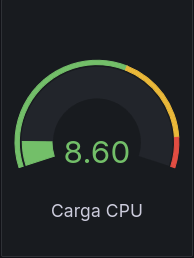
\includegraphics[width=0.3\linewidth]{cargaCPU.png}
    \caption{Carga de CPU}
    \label{fig:carga-cpu}
\end{figure}
\newpage

\subsection{Frecuencia de CPU}

La frecuencia instantánea de la CPU se muestra en el panel de Grafana bajo la visualización ``Gauge''. Esta visualización ha sido elegida porque representa de forma clara la frecuencia de operación del procesador en MHz, permitiendo comparar su estado actual con un valor máximo predefinido.\

Está configurado para mostrar el valor exacto de la frecuencia y una semicircunferencia que va desde 0 hasta 4000 MHz. Se ha supuesto 4000 MHz como frecuencia máxima de la CPU debido a que la media suele ser 2000 MHz y la máquina virtual no proporcionaba un valor máximo. La visualización cambia de color según el porcentaje de la frecuencia de la CPU: verde del 0\% al 80\%, amarillo del 80\% al 90\%, y rojo del 90\% al 100\% del valor máximo de frecuencia (4000 MHz).\

La consulta utilizada es la siguiente:

\begin{lstlisting}[language=SQL]
SELECT frecuencia FROM grafana.cpu;
\end{lstlisting}

Esta consulta selecciona el campo `frecuencia` de la tabla `cpu`, obteniendo la frecuencia actual del procesador. Esto permite a los administradores verificar si la CPU está funcionando dentro de los rangos esperados o si está alcanzando valores críticos.\

\begin{figure}[h!]
    \centering
    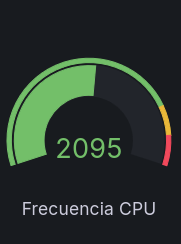
\includegraphics[width=0.3\linewidth]{frecuenciaCPU.png}
    \caption{Frecuencia de CPU}
    \label{fig:frecuencia-cpu}
\end{figure}

\subsection{Uso de memoria RAM y memoria SWAP}

El uso de memoria RAM y SWAP se muestra en el panel de Grafana bajo una visualización ``Time Series'', ya que permite observar la evolución del uso de ambas a lo largo del tiempo. Este tipo de visualización permite identificar tendencias y detectar posibles picos de uso que podrían afectar el rendimiento del sistema. Además se muestran tanto los valores mínimos y máximos que se han alcanzando en ambos usos de memoria.\

La consulta SQL utilizada para obtener estos valores es:

\begin{lstlisting}[language=SQL]
SELECT ram, swap, timestamp FROM grafana.memoria 
WHERE timestamp >= now() - interval 5 minute
ORDER BY timestamp ASC;
\end{lstlisting}

Aquí se seleccionan los valores de `ram` y `swap`, junto con la marca de tiempo `timestamp`, filtrando solo los datos de los últimos cinco minutos y ordenándolos cronológicamente. Esto permite visualizar cómo ha cambiado el uso de la memoria en ese período de tiempo.\

\begin{figure}[!h]
    \centering
    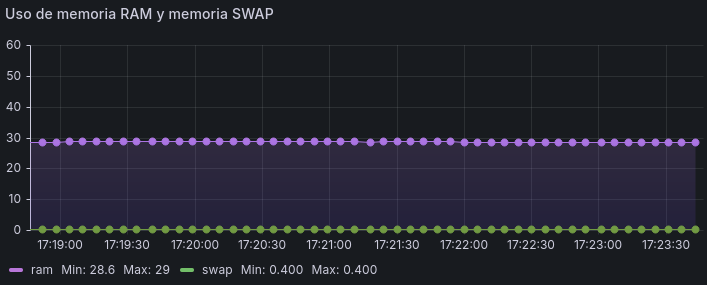
\includegraphics[width=0.9\linewidth]{memoria.png}
    \caption{Uso de memoria RAM y Swap}
    \label{fig:enter-label}
\end{figure}

\subsection{Espacio en disco}

El espacio en disco se muestra en el panel de Grafana bajo una visualización ``Pie Chart'', que permite visualizar el porcentaje de disco utilizado y el espacio libre en tiempo real. Este tipo de gráfico es elegido ya que permite ver de forma clara la proporción de almacenamiento consumido frente al disponible.\

El gráfico está configurado para mostrar en verde el espacio utilizado y en amarillo el espacio libre. Además, en la gráfica se incluyen los porcentajes exactos con números.\

La consulta SQL utilizada es:

\begin{lstlisting}[language=SQL]
SELECT espacio as "Usado", 100 - espacio as "Libre" FROM grafana.disco;
\end{lstlisting}

Esta consulta calcula dinámicamente el espacio libre restando el valor `espacio` (usado) de 100, proporcionando así un desglose claro del almacenamiento.\

\begin{figure}[!h]
    \centering
    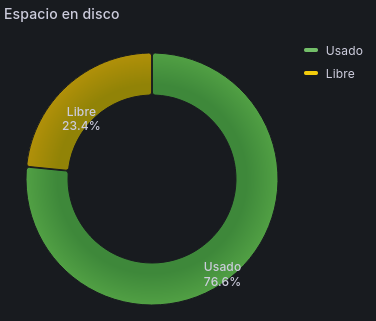
\includegraphics[width=0.5\linewidth]{disco.png}
    \caption{Espacio en Disco}
    \label{fig:enter-label}
\end{figure}
\newpage
\subsection{Operaciones de E/S}

Las operaciones de entrada y salida (E/S) se muestran en el panel de Grafana con una visualización ``Time Series'' en formato de gráfico de barras. Esta elección permite ver la cantidad de operaciones de lectura y escritura en diferentes momentos del tiempo, facilitando la identificación de posibles cuellos de botella en el sistema de almacenamiento.\

\begin{lstlisting}[language=SQL]
SELECT * FROM grafana.entradasalida 
WHERE timestamp >= now() - interval 5 minute
ORDER BY timestamp ASC;
\end{lstlisting}

Esta consulta recupera todas las columnas de la tabla `entradasalida` para los últimos cinco minutos, lo que permite analizar la actividad reciente del disco.\

\begin{figure}[!h]
    \centering
    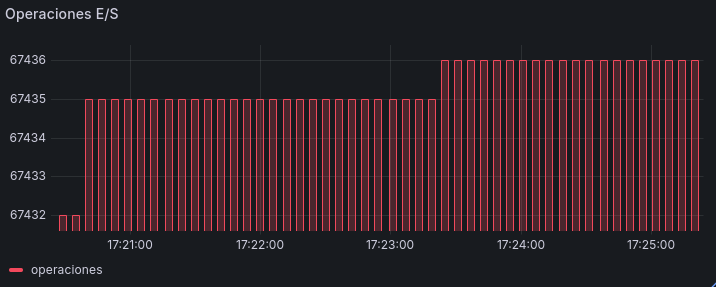
\includegraphics[width=0.9\linewidth]{operaciones.png}
    \caption{Operaciones de E/S}
    \label{fig:enter-label}
\end{figure}

\subsection{Bytes enviados y recibidos}

Los bytes enviados y recibidos se muestran en Grafana en paneles de tipo ``Time Series'' con un gráfico de líneas. Esta representación facilita el seguimiento del tráfico de red a lo largo del tiempo. Además se muestran los últimos bytes tanto enviados como recibidos y la suma total de todos.\

\begin{lstlisting}[language=SQL]
SELECT bytes_enviados, timestamp FROM grafana.red
WHERE timestamp >= now() - interval 5 minute
ORDER BY timestamp ASC;

SELECT bytes_recibidos, timestamp FROM grafana.red
WHERE timestamp >= now() - interval 5 minute
ORDER BY timestamp ASC;
\end{lstlisting}

Estas consultas seleccionan los bytes enviados y recibidos en los últimos cinco minutos, permitiendo detectar patrones de uso y posibles congestiones en la red.\

\begin{figure}[!h]
    \centering
    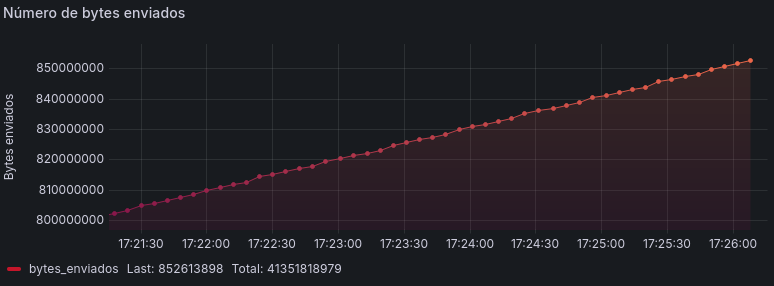
\includegraphics[width=0.9\linewidth]{bytes_enviados.png}
    \caption{Bytes enviados}
    \label{fig:enter-label}
\end{figure}

\begin{figure}[!h]
    \centering
    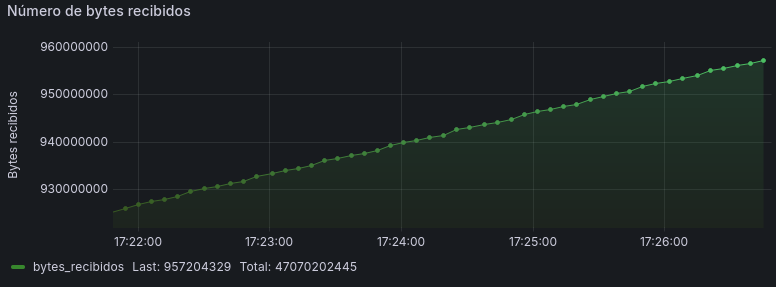
\includegraphics[width=0.9\linewidth]{bytes_recibidos.png}
    \caption{Bytes recibidos}
    \label{fig:enter-label}
\end{figure}
\newpage
\subsection{Conexiones de red activas}

Las conexiones de red activas se muestran en Grafana en un panel de tipo ``Stat'', el cual permite visualizar las conexiones activas en un instante dado. También permite observar picos en los que hubo mayor número de conexiones de red. A medida que aumenta la cantidad de conexiones, las tonalidades de color varían.\

\begin{lstlisting}[language=SQL]
SELECT conexiones_activas as "Conexiones Activas" FROM grafana.red;
\end{lstlisting}

Esta consulta obtiene el número de conexiones activas en tiempo real, lo que facilita la supervisión del tráfico en la red.\

\begin{figure}[!h]
    \centering
    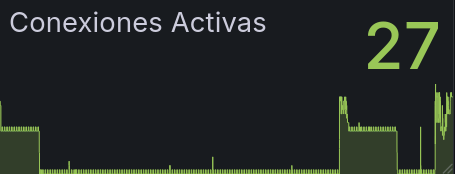
\includegraphics[width=0.6\linewidth]{conexiones_activas.png}
    \caption{Conexiones de red Activas}
    \label{fig:enter-label}
\end{figure}

\subsection{Número de procesos en ejecución}

El número de procesos en ejecución se muestra en Grafana en un panel de tipo ``Stat'', que permite visualizar la cantidad de procesos activos en un instante dado.\

\begin{lstlisting}[language=SQL]
SELECT numero, timestamp FROM grafana.num_procesos;
\end{lstlisting}

Esta consulta proporciona el número actual de procesos, útil para detectar posibles sobrecargas en el sistema.\

\begin{figure}[!h]
    \centering
    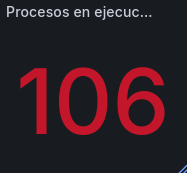
\includegraphics[width=0.3\linewidth]{procesos_ejecc.png}
    \caption{Procesos en ejecución}
    \label{fig:enter-label}
\end{figure}
\newpage
\subsection{Lista detallada de los procesos en ejecución}

La lista de procesos en ejecución se muestra en Grafana en una tabla, lo que permite acceder, visualizar y filtrar todos los procesos en tiempo real junto con sus detalles.\

\begin{lstlisting}[language=SQL]
SELECT usuario as Usuario, pid as PID, 
cpu_percent as CPU, memory_percent as MEM, vsz as VSZ, rss as RSS, estado as Stat, 
nombre as Nombre, ruta as Comando, hilos as hilos FROM 
grafana.procesos;
\end{lstlisting}
Esta consulta obtiene una lista detallada de los procesos en ejecución en el sistema como lo haria el comando \textbf{ps aux} de Linux:
\begin{itemize}
    \item \textbf{usuario}: Indica el usuario que ha iniciado el proceso.
    \item \textbf{pid}: Identificador único del proceso.
    \item \textbf{cpu\_percent}: Porcentaje de uso de CPU del proceso.
    \item \textbf{memory\_percent}: Porcentaje de uso de memoria RAM.
    \item \textbf{vsz}: Tamaño virtual del proceso en memoria.
    \item \textbf{rss}: Tamaño real del proceso en RAM.
    \item \textbf{estado}: Estado actual del proceso (ejecución, suspensión, etc.).
    \item \textbf{nombre}: Nombre del proceso.
    \item \textbf{ruta}: Ruta de ejecución del proceso o nombre del comando (en este caso coincidirá con el nombre del proceso).
    \item \textbf{hilos}: Número de hilos asociados al proceso.
\end{itemize}
Esta información es útil para el monitoreo del sistema, ya que permite detectar procesos que consumen muchos recursos y podrían estar afectando el rendimiento del sistema.

\begin{figure}[!h]
    \centering
    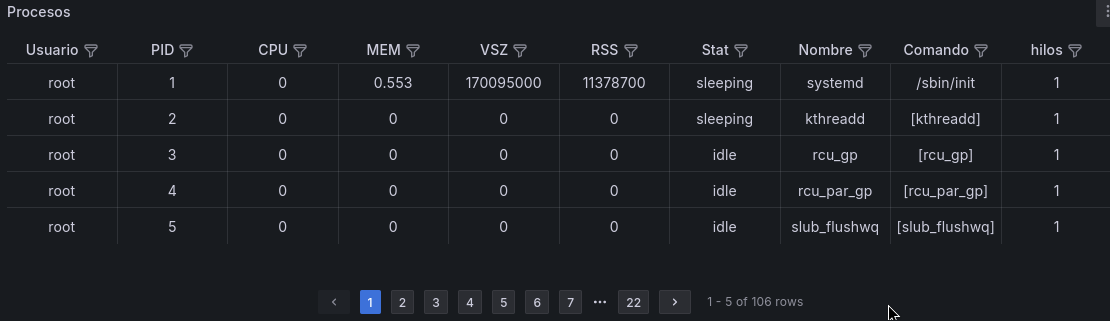
\includegraphics[width=1.3\linewidth]{procesos.png}
    \caption{Detalles de los procesos en ejecución}
    \label{fig:enter-label}
\end{figure}
\newpage

\section{Distribuciónde trabajo y organización}

\section{Bibliografia}
\end{document}